\documentclass[12pt]{article}
\usepackage{amsmath, amssymb, amsthm}
\usepackage{geometry}
\usepackage{hyperref}
\usepackage{listings}
\usepackage{xcolor}
\usepackage{graphicx}
\graphicspath{{./}{HW2/}}
\usepackage{booktabs}
\usepackage{array}
\usepackage{tabularx}
\usepackage{placeins}
\usepackage{tikz}
\usetikzlibrary{arrows.meta, positioning}
\definecolor{stageblue}{HTML}{307BF3}

\geometry{margin=1in}

\lstset{
    language=Python,
    basicstyle=\ttfamily\small,
    keywordstyle=\color{blue},
    stringstyle=\color{red},
    commentstyle=\color{green!50!black},
    showstringspaces=false,
    breaklines=true,
    frame=single,
    numbers=left,
    numberstyle=\tiny
}

\title{From Clicks to Vectors: The Geometry of Recommendation}
\author{XIA JIAHAN}
\date{\today}

\begin{document}
\maketitle

\section{Recommendation Motivation}

In the information explosion era, recommendation systems (RS) are essential for filtering vast data and delivering personalized content across platforms like Amazon, Netflix, YouTube, and social media, enhancing user experience and business value by predicting preferences. They use machine learning to model similarities between items and user interests, powering two main types of suggestions: personalized homepage feeds (unique to each user) and related item recommendations (e.g., suggesting science apps when viewing a math app). This enables platforms like YouTube and the Google Play Store to anticipate what to show next. The core motivation is to help users navigate immense content libraries, where search alone falls short, by surfacing relevant, sometimes unexpected items and facilitating discovery.

A recommender system matches a user's query (context) to recommendable entities (items) by learning embeddings that place queries and items in a shared vector space for efficient similarity computation. It then performs candidate generation to quickly narrow a huge corpus to hundreds or thousands of candidates, scoring to rank this smaller set and select roughly ten items to display, and finally re-ranking to apply constraints such as removing content the user dislikes, boosting fresher items, and ensuring diversity and fairness. We will discuss each stage with examples from systems like YouTube.

\begin{figure}[htbp]
    \centering
    \resizebox{\linewidth}{!}{%
    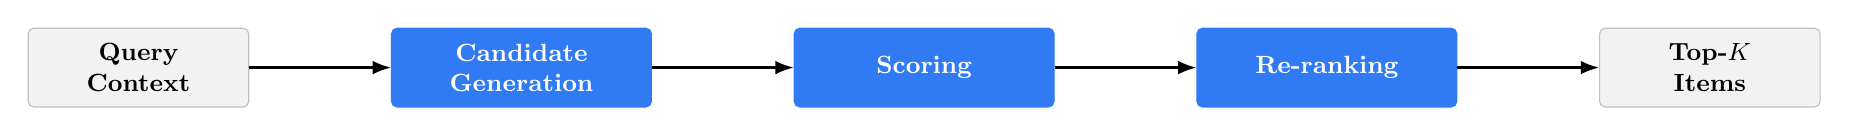
\begin{tikzpicture}[
        node distance=1.8cm,
        >=Latex,
        stage/.style={draw=stageblue, fill=stageblue, rounded corners=2pt, text=white, font=\small\bfseries, minimum height=10mm, minimum width=33mm, align=center},
        io/.style={draw=black!25, fill=black!5, rounded corners=2pt, font=\small\bfseries, minimum height=10mm, minimum width=28mm, align=center}
    ]
        \node[io] (query) {Query\\Context};
        \node[stage, right=of query] (cand) {Candidate\\Generation};
        \node[stage, right=of cand] (score) {Scoring};
        \node[stage, right=of score] (rerank) {Re-ranking};
        \node[io, right=of rerank] (results) {Top-$K$\\Items};

        \draw[->, thick] (query) -- (cand);
        \draw[->, thick] (cand) -- (score);
        \draw[->, thick] (score) -- (rerank);
        \draw[->, thick] (rerank) -- (results);
    \end{tikzpicture}%
    }
    \caption{Overview of the Recommender System Process}
    \label{fig:process_flow}
\end{figure}

\section{Candidate Generation}
Candidate generation is the first stage of recommendation. Given a query, the system generates a set of relevant candidates. The following table shows two common candidate generation approaches:

\begin{table}[ht]
    \centering
    \renewcommand{\arraystretch}{1.2}
    \begin{tabularx}{\linewidth}{l X X}
        \toprule
        Type & Definition & Example \\
        \midrule
        content-based filtering & Uses \emph{similarity between items} to recommend items similar to what the user likes. & If user A watches two cute cat videos, then the system can recommend cute animal videos to that user. \\
        \midrule
        collaborative filtering & Uses \emph{similarities between queries and items simultaneously} to provide recommendations. & If user A is similar to user B, and user B likes video 1, then the system can recommend video 1 to user A (even if user A hasn't seen any videos similar to video 1). \\
        \bottomrule
    \end{tabularx}
\end{table}

Both content-based and collaborative filtering embed items and queries (contexts) into a shared low-dimensional space \(E=\mathbb{R}^{d}\). Candidate generation then retrieves items whose embeddings are most similar to the query embedding: a similarity function \(s:E\times E\to\mathbb{R}\) ranks candidates by \(s(q,x)\). Common choices include cosine similarity, dot product, and Euclidean distance.

Unlike cosine similarity, dot product is sensitive to embedding norms, so large-norm vectors can be preferred even when the angle is similar. This can affect recommendations as follows:
\begin{itemize}
    \item Popular items often get large norms, so dot product can capture popularity but may cause popular items to dominate. A tempered variant is \(s(q,x)=\lVert q\rVert^{\alpha}\,\lVert x\rVert^{\alpha}\,\cos(q,x)\) for \(\alpha\in(0,1)\).
    \item Rare items may be updated infrequently; if initialized with large norms they can be over-recommended. To avoid this problem, be careful about embedding initialization and use appropriate regularization.
\end{itemize}

\section{Content Based Filtering}

Content-based filtering recommends items that are similar to what a user already likes by comparing item feature vectors. For example, one can build a simple (binary) feature matrix for apps; a user can be represented in the same feature space using explicit preferences and past installs. Given a similarity metric (e.g., dot product), the system scores each candidate item against the user vector and recommends the highest-scoring items, without using information from other users.

Content-based filtering has the advantage that it does not require data about other users, since recommendations are computed specifically for a given user, which makes it easier to scale to a large user base; it can also capture a user’s particular interests and recommend niche items that few other users care about. However, it often relies on partially hand-engineered item features and substantial domain knowledge, so performance is limited by the quality of those features, and it can only recommend based on the user’s existing interests, giving it limited ability to broaden the user’s preferences beyond what they have already shown.

\section{Collaborative Filtering}
To address some of the limitations of content-based filtering, collaborative filtering uses similarities between users and items simultaneously to provide recommendations. This allows for serendipitous recommendations; that is, collaborative filtering models can recommend an item to user A based on the interests of a similar user B. Furthermore, the embeddings can be learned automatically, without relying on hand-engineering of features.

In practice, one of the most common ways to implement collaborative filtering is to \emph{learn embeddings} for users and items. The idea is to represent each user \(j\) by a vector \(u_j\) and each movie \(i\) by a vector \(v_i\), and then use a simple similarity score (often a dot product \(u_j^\top v_i\)) to predict whether the user will interact with the movie. This directly explains why embeddings are central to candidate generation: once users and items live in the same vector space, nearest-neighbor search can efficiently retrieve relevant items at scale.

Consider a movie recommendation system in which the training data consist of a feedback matrix in which:
\begin{itemize}
    \item Each row represents a user.
    \item Each column represents an item (a movie).
\end{itemize}

The feedback about movies falls into one of two categories:
\begin{itemize}
    \item \textbf{Explicit}---users specify how much they liked a particular movie by providing a numerical rating.
    \item \textbf{Implicit}---if a user watches a movie, the system infers that the user is interested.
\end{itemize}

To simplify, we assume that the feedback matrix is binary; that is, a value of \(1\) indicates interest in the movie. When a user visits the homepage, the system should recommend movies based on both:
\begin{itemize}
    \item similarity to movies the user has liked in the past;
    \item movies that similar users liked.
\end{itemize}

This is the bridge from collaborative filtering to embeddings. Collaborative filtering can be viewed as learning low-dimensional vectors \(u_j\) (users) and \(v_i\) (items) so that their dot product predicts interest; in matrix form, this is a low-rank approximation of the sparse feedback matrix. Once these vectors are learned, they live in a shared embedding space, and candidate generation becomes a nearest-neighbor search: for a user/query vector, retrieve items whose embeddings are most similar.

To make the connection concrete, we will use a small set of movies (Table below) and visualize what it means to embed movies and users in 1D and 2D.

\begin{table}[ht]
    \centering
    \renewcommand{\arraystretch}{1.15}
    \begin{tabularx}{\linewidth}{>{\raggedright\arraybackslash}p{0.25\linewidth} c X}
        \toprule
        Movie & Rating & Description \\
        \midrule
        The Dark Knight Rises & PG-13 & Batman endeavors to save Gotham City from nuclear annihilation in this sequel to \emph{The Dark Knight}, set in the DC Comics universe. \\
        \midrule
        Harry Potter and the Sorcerer's Stone & PG & An orphaned boy discovers he is a wizard and enrolls in Hogwarts School of Witchcraft and Wizardry, where he wages his first battle against the evil Lord Voldemort. \\
        \midrule
        Shrek & PG & A lovable ogre and his donkey sidekick set off on a mission to rescue Princess Fiona, who is imprisoned in her castle by a dragon. \\
        \midrule
        The Triplets of Belleville & PG-13 & When professional cyclist Champion is kidnapped during the Tour de France, his grandmother and overweight dog journey overseas to rescue him, with the help of a trio of elderly jazz singers. \\
        \midrule
        Memento & R & An amnesiac desperately seeks to solve his wife's murder by tattooing clues onto his body. \\
        \bottomrule
    \end{tabularx}
\end{table}
\FloatBarrier

\section{Embeddings}
With collaborative filtering, the key modeling choice is to replace sparse user--movie interactions by dense vectors that can be compared reliably. An \emph{embedding} represents an entity (a movie, a user, or a query context) as a vector in a low-dimensional Euclidean space \(E=\mathbb{R}^d\). The goal is to place entities so that geometric proximity (or a similarity score) reflects behavioral similarity. In collaborative filtering, this is typically done by assigning
\[
u_j \in \mathbb{R}^d \quad \text{to user } j,
\qquad
v_i \in \mathbb{R}^d \quad \text{to movie } i,
\]
and scoring user--movie affinity by a dot product
\[
\widehat{r}_{j i} \;=\; u_j^\top v_i,
\]
so that large scores correspond to likely interest.

\subsection{One Dimensional Embeddings}
In the 1D picture (Figure~\ref{fig:embed_1d}), each user and each movie is represented by a single scalar in \(\mathbb{R}\). Geometrically, that is a point on a line. Conceptually, you can interpret the line as one dominant latent factor, for example a spectrum from ``children'' to ``adult''. A movie on the left is more ``children-oriented'', and a movie on the right is more ``adult-oriented''. A user’s scalar indicates which side of the spectrum they tend to prefer.

In 1D, the dot product reduces to multiplication: \(\widehat{r}_{ji} = u_j v_i\). A user and a movie with the same sign (both on the left or both on the right) get a positive score; opposite signs yield a negative score. This explains why, in a 1D embedding, the model can capture a single dominant preference trend but cannot separate different reasons for liking something.

\begin{figure}[htbp]
    \centering
    \begin{minipage}[t]{0.49\linewidth}
        \centering
        \includegraphics[width=\linewidth]{1D.png}
        \vspace{0.25em}
        
        {\small (a) 1D geometry: movies and users on a line.}
    \end{minipage}\hfill
    \begin{minipage}[t]{0.49\linewidth}
        \centering
        \includegraphics[width=\linewidth]{1Dmatrix.png}
        \vspace{0.25em}
        
        {\small (b) 1D parameters: one scalar embedding per entity.}
    \end{minipage}
    \caption{A 1D embedding: each movie/user is represented by one number in \(\mathbb{R}\).}
    \label{fig:embed_1d}
\end{figure}
\FloatBarrier

\subsection{Two Dimensional Embeddings}
The 2D picture (Figure~\ref{fig:embed_2d}) assigns each user and movie a vector in \(\mathbb{R}^2\). Geometrically, that is a point in the plane. Now the model can represent \emph{two} latent factors at once. One axis can still align with ``children vs.\ adult'', while the second axis can capture something different, such as ``blockbuster vs.\ arthouse'' style. This resolves a key limitation of 1D: two movies that were forced to sit near each other on a line can be separated in the plane because the model has an extra degree of freedom.

Algebraically, the score becomes \(\widehat{r}_{ji} = u_j^\top v_i\) with \(u_j, v_i \in \mathbb{R}^2\). The matrix in Figure~\ref{fig:embed_2d} shows the same idea in parameter form: each user and each movie now has two coordinates. In practice, recommendation systems use higher-dimensional embeddings (\(d\) in the tens to thousands), but the geometric intuition is the same as in 2D: more dimensions allow the model to encode more independent preference factors.

\begin{figure}[htbp]
    \centering
    \begin{minipage}[t]{0.49\linewidth}
        \centering
        \includegraphics[width=\linewidth]{2D.png}
        \vspace{0.25em}
        
        {\small (a) 2D geometry: movies and users in a plane.}
    \end{minipage}\hfill
    \begin{minipage}[t]{0.49\linewidth}
        \centering
        \includegraphics[width=\linewidth]{2Dmatrix.png}
        \vspace{0.25em}
        
        {\small (b) 2D parameters: a 2D embedding vector per entity.}
    \end{minipage}
    \caption{A 2D embedding: each movie/user is represented by a vector in \(\mathbb{R}^2\), enabling the model to capture more than one latent factor.}
    \label{fig:embed_2d}
\end{figure}
\FloatBarrier

\subsection{Matrix Factorization}
Let \(A \in \mathbb{R}^{m \times n}\) be the feedback matrix, where \(m\) is the number of users and \(n\) is the number of items. Matrix factorization seeks two low-dimensional embedding matrices
\[
U \in \mathbb{R}^{m \times d}, \qquad V \in \mathbb{R}^{n \times d},
\]
such that \(A \approx U V^\top\). The predicted interaction is the dot product of the corresponding embeddings:
\[
\widehat{A}_{ij} = \langle U_i, V_j \rangle.
\]
This is a low-rank approximation: instead of storing \(O(mn)\) entries, the model stores \(O((m+n)d)\) parameters, with \(d \ll m,n\), which is crucial for large-scale systems.

An intuitive objective is squared error on observed interactions:
\[
\min_{U,V} \sum_{(i,j)\in \text{obs}} \big(A_{ij} - \langle U_i, V_j \rangle\big)^2.
\]
However, optimizing only on observed entries can lead to degenerate solutions (for example, predicting ones everywhere) and poor generalization. A different extreme is to treat \emph{all} unobserved entries as zeros and minimize \(\|A-UV^\top\|_F^2\), which corresponds to SVD; in very sparse data this tends to push predictions toward zero. A common fix is \emph{Weighted Matrix Factorization}, which treats unobserved entries as zeros but downweights them:
\[
\min_{U,V} \sum_{(i,j)\in \text{obs}} w_{ij}\big(A_{ij} - \langle U_i, V_j \rangle\big)^2
 \;+\; w_0 \sum_{(i,j)\notin \text{obs}} \langle U_i, V_j \rangle^2.
\]
The weights \(w_{ij}\) can correct for popularity (very active users or very popular items), while \(w_0\) balances observed and unobserved terms and must be tuned.

To minimize the objective, two standard choices are:
\begin{itemize}
    \item \textbf{SGD (stochastic gradient descent):} flexible and works with many loss functions, but can converge slowly and typically needs negative sampling for unobserved entries.
    \item \textbf{WALS (weighted alternating least squares):} alternates between fixing \(U\) and solving for \(V\), then fixing \(V\) and solving for \(U\). Each step solves a linear system, converges quickly, and handles unobserved entries naturally.
\end{itemize}

\subsection{Advantages and disadvantages of matrix factorization}
\paragraph{Advantages.}
\begin{itemize}
    \item \textbf{No domain knowledge necessary.} Embeddings are learned automatically from the feedback matrix, so the model does not require hand-crafted item features.
    \item \textbf{Serendipity.} The model can surface items a user has never interacted with, because similar users liked them. This enables discovery beyond the user's immediate history.
    \item \textbf{Great starting point.} A basic factorization model needs only the feedback matrix. It can serve as a strong baseline or one of multiple candidate generators without extra contextual features.
\end{itemize}

\paragraph{Disadvantages.}
\begin{itemize}
    \item \textbf{Cannot handle fresh items (cold-start).} For an unseen item, the model has no embedding, so it cannot score the item. Two common workarounds are:
    \begin{itemize}
        \item \textbf{Projection in WALS.} With a few interactions, solve a weighted least-squares problem for the new item's embedding:
        \[
        v_i \;=\; \arg\min_{v} \sum_{j} w_{ij}\big(A_{ij} - u_j^\top v\big)^2,
        \]
        which is one WALS step with user embeddings fixed. The same idea applies to new users.
        \item \textbf{Heuristic embeddings.} If there are no interactions, approximate the new item's embedding by averaging embeddings of related items (same category, same uploader, etc.).
    \end{itemize}
    \item \textbf{Hard to include side features.} Side features (e.g., country, age, device type, item metadata) often improve quality, but pure matrix factorization does not naturally incorporate them without extending the model.
\end{itemize}

\section{Retrieval}
With embeddings for users and items, retrieval (candidate generation) becomes a geometric search problem. At serve time, given a query, you start by doing one of the following:

For a matrix factorization model, the query (or user) embedding is known statically, and the system can simply look it up from the user embedding matrix.
For a DNN model, the system computes the query embedding $\psi(x) $ at serve time by running the network on the feature vector $x$. Once you have the query embedding $q$, search for item embeddings $V_j$
that are close to $q$ in the embedding space. This is a nearest neighbor problem. For example, you can return the top k items according to the similarity score $s(q,V_j) = \langle q, V_j \rangle$.

\begin{figure}[htbp]
    \centering
    \includegraphics[width=0.9\linewidth]{2Dretrieval.png}
    \caption{Retrieval in an embedding space.}
    \label{fig:retrieval_2d}
\end{figure}
\FloatBarrier

\section{Scoring}
Retrieval returns a manageable candidate set, but the similarity function used for fast nearest-neighbor search is usually too simple to make the final decision. The scoring stage applies a more expressive model to the retrieved candidates and estimates a utility for each item under the current context, for example
\[
\widehat{y} = f(q, v_i, x),
\]
where \(q\) is the query or user embedding, \(v_i\) is the candidate item embedding, and \(x\) collects additional features such as item metadata, freshness, device, and short-term session signals. Typical outputs include predicted click-through rate, watch time, or a multi-objective score that combines several engagement signals.

Compared with retrieval, scoring can afford heavier computation because it only evaluates hundreds or thousands of items. This is where models can use richer feature crosses, deeper networks, and better calibration, while still meeting latency constraints.

\section{Reranking}
Even a well-trained scoring model may not satisfy product constraints by itself. The reranking stage takes the top scored list and modifies it to enforce constraints and improve user experience. Common goals include:
\begin{itemize}
    \item \textbf{Diversity:} avoid showing many near-duplicates by penalizing redundant items.
    \item \textbf{Freshness:} boost newer items when appropriate.
    \item \textbf{Safety and filtering:} remove items the user dislikes or content that violates policy.
    \item \textbf{Business constraints:} apply quotas, category balance, or exploration requirements.
\end{itemize}
Conceptually, reranking can be viewed as optimizing a final objective that trades off relevance (scores) against constraint penalties, often implemented by a greedy selection procedure over the scored candidates.

\end{document}
